\documentclass{beamer}
\usepackage{framed}
\usetheme[pageofpages=of,% String used between the current page and the
                         % total page count.
          bullet=circle,% Use circles instead of squares for bullets.
          titleline=true,% Show a line below the frame title.
          alternativetitlepage=true,% Use the fancy title page.
          ]{Torino}

\setbeamercovered{invisible}          
\setbeamertemplate{section page}
{
	\huge{\insertsection}
	 \textcolor{chameleongreen3}{\hrule height 1pt} 	
  	\vspace{0px}
}  
\usepackage{pifont}
\usepackage[utf8]{inputenc}
\usepackage{multicol}


\newcommand{\hiddencell}[2]{\action<#1->{#2}}
% first argument: slide number to appear from, second argument: content of cell        

\author[Otto, Döring, Kiessling]{Wolfgang Otto, Thomas Döring, Max Kießling}
\title{Wortschatz Zeitgeist}
\institute{Seminar Anwendungen der linguistischen Informatik}
\date{16. Juni 2015}

\begin{document}	
\watermarkoff

\begin{frame}[t,plain]
	\titlepage
\end{frame}

\begin{frame}[t,plain]
	\tableofcontents
\end{frame}


\section{Motivation}
\begin{frame} \sectionpage \end{frame}


\begin{frame}{Wortschatzprojekt}
 \begin{itemize}
 	\item Bla
 	\item Foobar
 	\item Batz
 \end{itemize}
 
 \begin{definition}
 	Definition
 \end{definition}
 
 \begin{example}
 	Beispiel
 \end{example}
\end{frame}


\section{Algorithmen}
\begin{frame} \sectionpage \end{frame}

\begin{frame}{Relative Häufigkeit}
	Something about relative frequency
\end{frame}

\begin{frame}{TF/IDF}
 	Something about TF/IDF
\end{frame}

\begin{frame}{Poison}
	Something about poison
\end{frame}

\begin{frame}{Z-Score}
	Something about Z-score
\end{frame}

\begin{frame}{Zeitreihenanalyse}
 \begin{definition}[Zeitreihenanalyse]
 	Unter einer Zeitreihe
	versteht man die Entwicklung einer bestimmten Größe, deren Werte im Zeitablauf zu bestimmten Zeitpunkten oder für bestimmte Zeitintervalle erfasst und dargestellt
	werden
 \end{definition}
	
\end{frame}

\begin{frame}{Maß: gleitender Mittelwert}
	\begin{itemize}
		\item Glättet Zeit oder Datenreihen
		\item Erfolgt durch glätten hoher Frequenzanteile
		\item Es gibt ein Raster der größe n		
		\item Es werden n Tage zusammenaddiert und dann durch n geteilt
	\end{itemize}
	
	Wie hilft uns das weiter?
	
	\begin{itemize}
		\item Tritt ein Wort häufiger als sein Durchschnittswert an dem Tag auf kann das interessant sein.
	\end{itemize}		
	
\end{frame}

\begin{frame}{Erster Ansatz: R}
	\begin{itemize}
		\item Der erste Ansatz war ein R Programm welches den gleitenden Mittelwert ausrechnen sollte
		\item Problem: R verarbeitet Wörter einzeln 
		\item 3 Mio. Wörter $\rightarrow$ 3 Mio. Transaktionen = MySQL Overkill
		\item Ausführungszeit würde mehrere Tage beanspruchen
	\end{itemize}
\end{frame}

\begin{frame}{Beispiel}
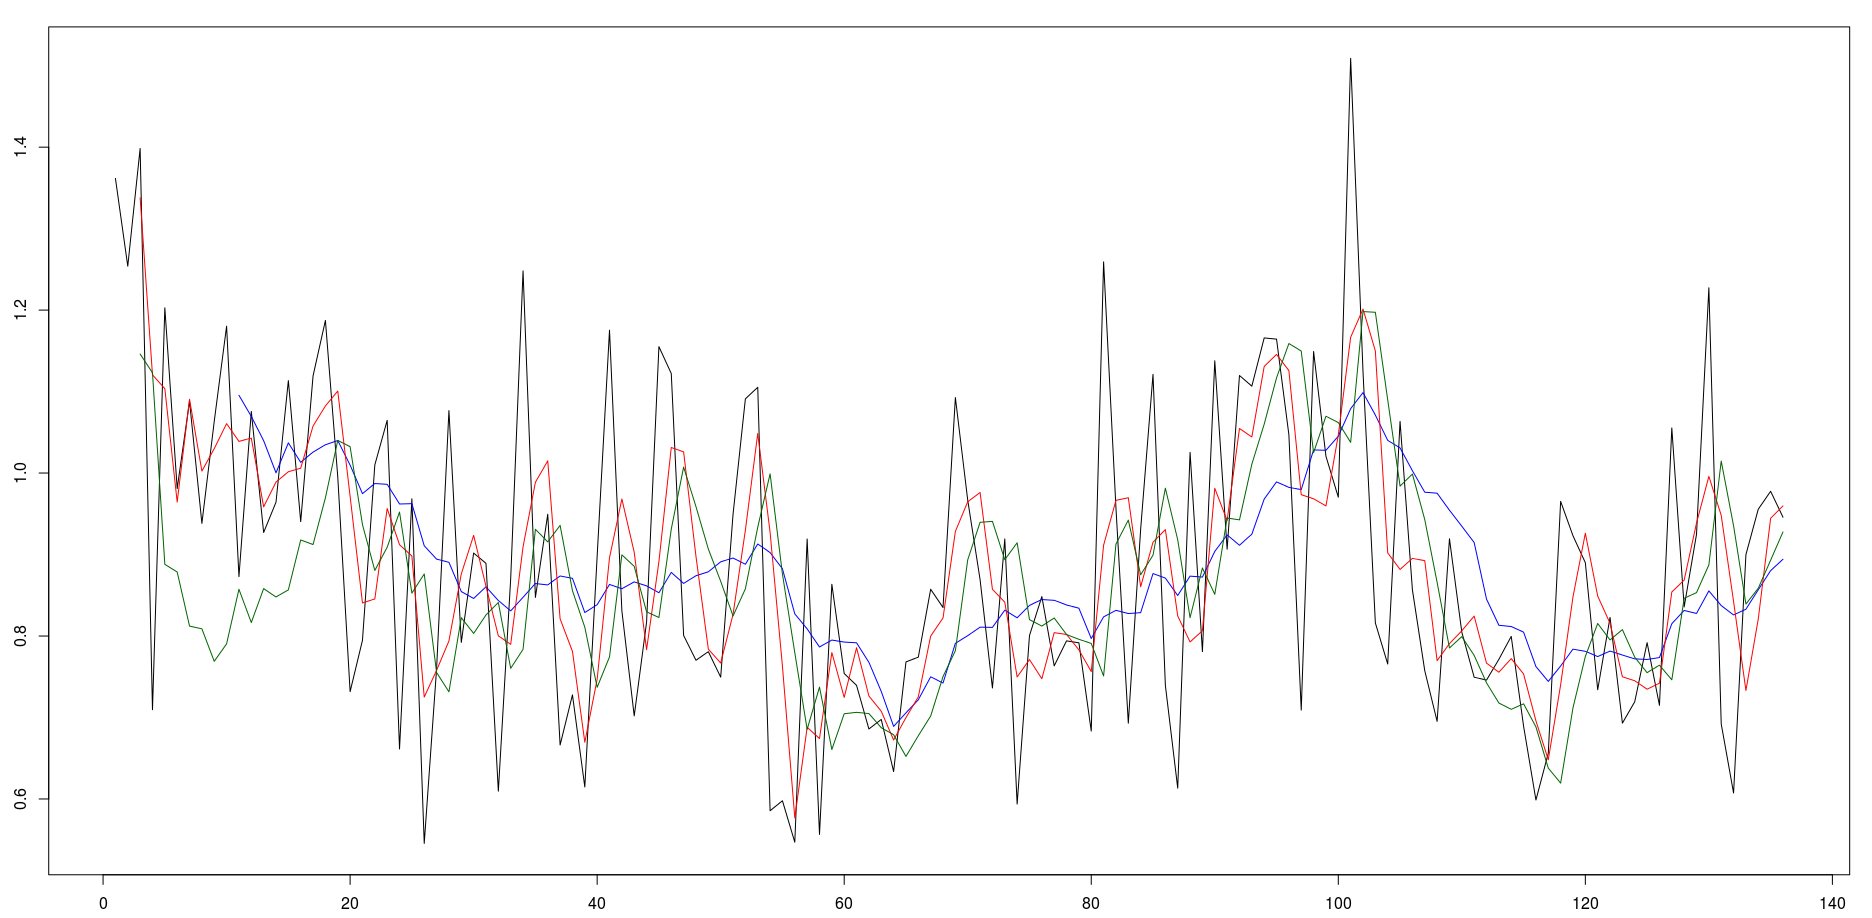
\includegraphics[scale=0.18]{Bilder/R.png}
\end{frame}

\begin{frame}{Zweiter Ansatz: MySQL}
	\begin{itemize}
		\item Der Zweite Ansatz ist es direkt in MySQL zu berechnen
		\item Problem: Inner Join auf selbe Tabelle (ca. 20 Mio Zeilen)
		\item Jeder Eintrag muss geprüft werden ob die Join Tabelle den Eintrag in der Größe des Rasters hat
		\item Eine Datums Differenz Tabelle kann das ganze jedoch beschleunigen

	\end{itemize}
\end{frame}

\section{Vergleich und Auswertung}
\begin{frame} \sectionpage \end{frame}

\begin{frame}{Zusammenfassung}
\end{frame}



\begin{frame}[allowframebreaks]{Quellen}
	\nocite{*}
	\bibliographystyle{plaindin}
    \bibliography{quellen}
\end{frame}

\end{document}